\section[波函数的统计诠释]{波函数的统计诠释} \label{sec:02.02} % 
% \makebox[5em][s]{} % 短题目拉间距

薛定谔方程中的波函数中,$\varPsi$一般是复数,因此$\varPsi$不可能直接描述某种物理量,波函数的确切含义,在量子力学建立以后才弄明白.

还是从光子说起.用单色光做圆孔衍射实验,如图\ref{fig.2-1}所示.屏上出现的衍射图样(明暗相间的衍射环)是光具有波动性的确证.屏上各处(以及由孔至屏整个空间)衍射光的亮度和衍射波的强度(波函数的模方,即$|\varPsi|^{2}$)成正比.强度大处为亮环,强度小处为暗环.衍射图样的形状(亮环和暗环的位置)完全取决于光波波长$\lambda$及孔的半径以及孔至屏的距离,而和入射光的总强度无关.可见,衍射并非各个光子互相影响所造成,而是每个光子的运动规律,光的波动性体现在每个光子上.但就一个光子来说,衍射后它总只能出现在屏上某个地方,而不可能同时出现在几个地方.显然,一个光子在屏上某处出现的概率和该处衍射波的强度成正比.光波强度($|\varPsi|^{2}$)大的地方,到达的光子总数多,亮度大;光波强度小的地方,到达的光子总数少,亮度小.
\begin{figure}[!h]
	\centering
	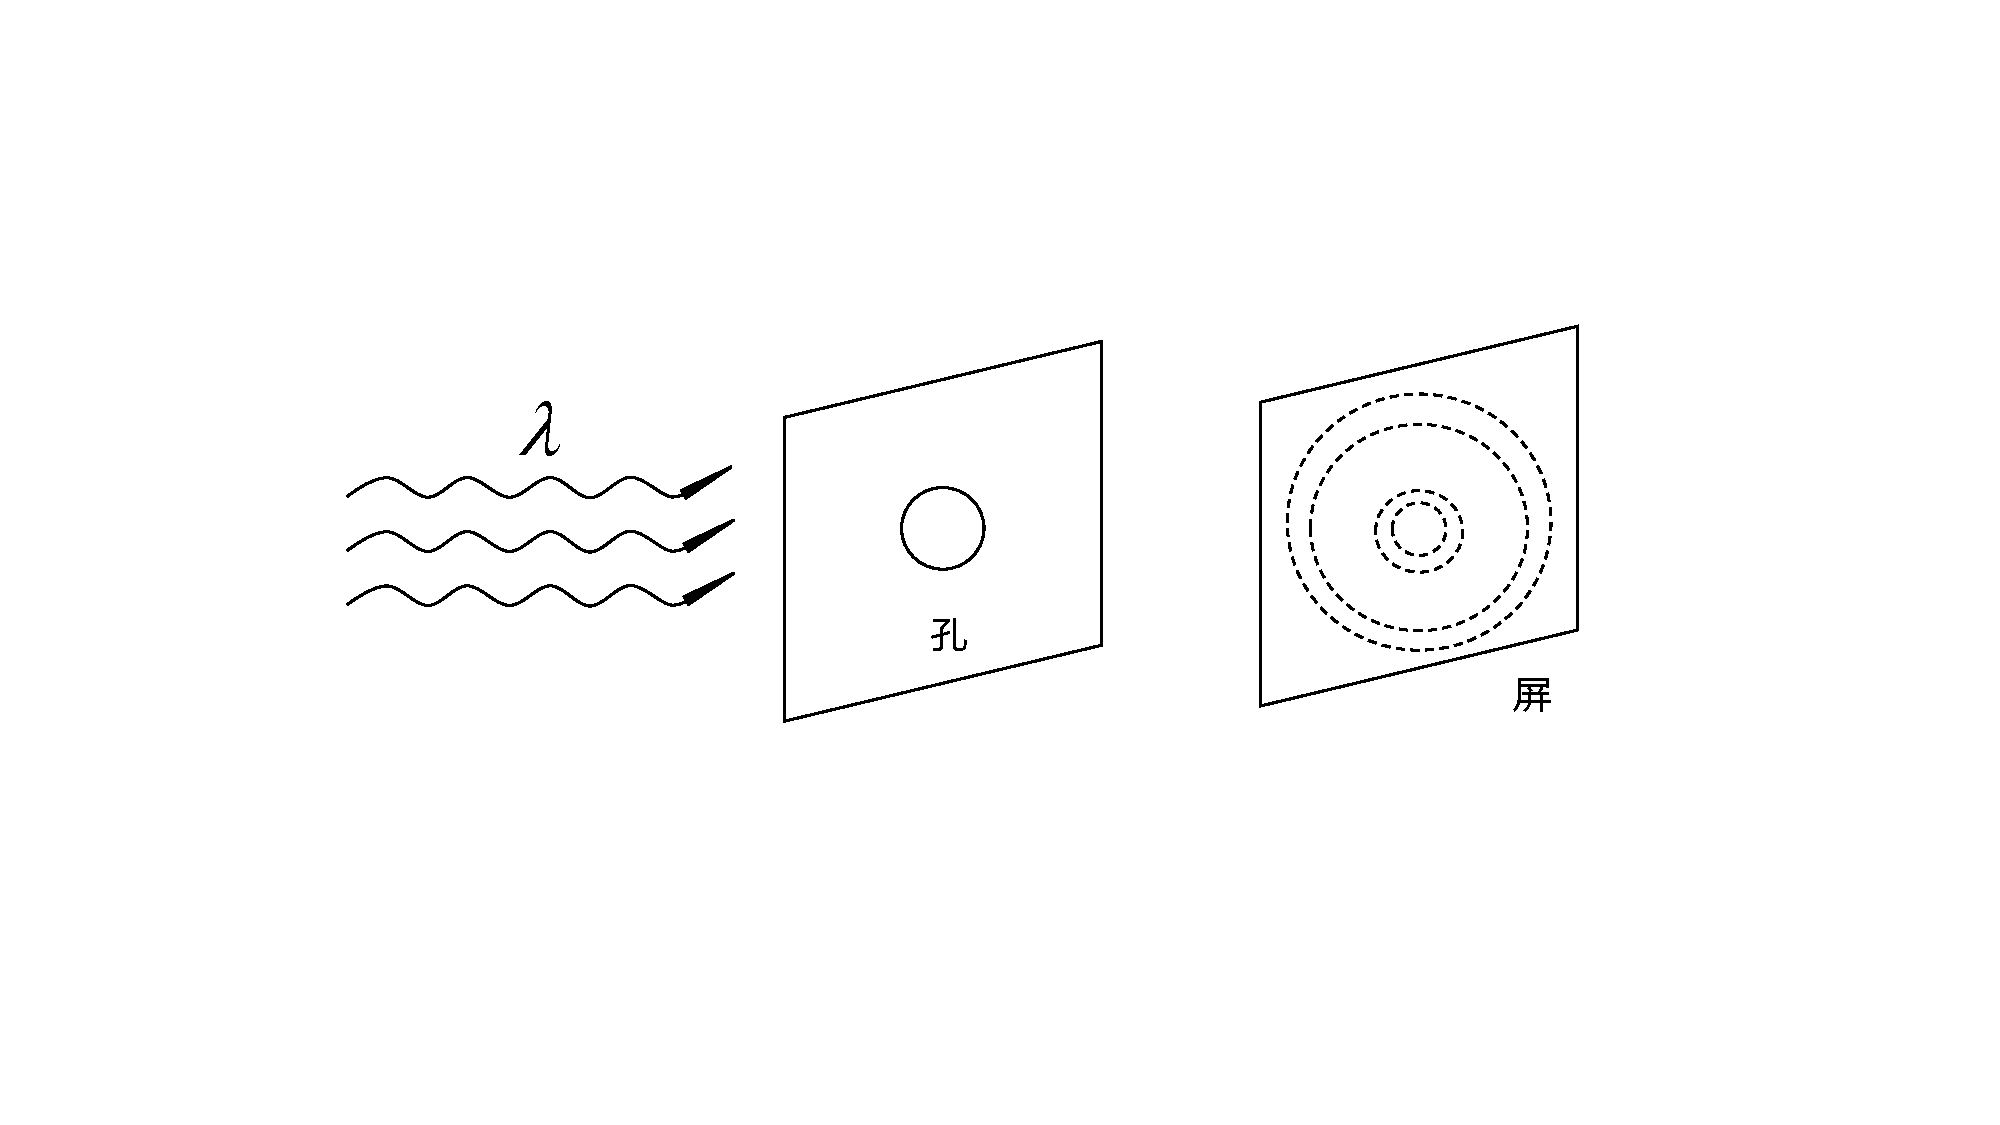
\includegraphics[width=5cm,clip]{QM file/figure/2-1}
	\caption{}\label{fig.2-1}
\end{figure}

用电子束代替光束进行的电子衍射实验结果类似,衍射图样取决于入射电子束的波长($\lambda=\frac{h}{p}$),而与电子总流量无关,这表明波动性是每一个电子的运动属性就一个电子来说,衍射后它将出现在屏上何处,事先无法预测,带有概率性;大量电子衍射的结果(相当于同样条件下单个电子衍射的多次重复),则表现出一定的规律性,屏上某处出现的电子总数和该处衍射波的(波函数的模方$|\varPsi|^{2}$)强度成正比.

基于这种认识,玻恩(M. Born)对薛定谔方程中的波函数提出了如下的统计诠释:
\eqlong
\begin{equation*}
	|\varPsi(\boldsymbol{r},t)|^{2} d\tau \propto \text{粒子在}t\text{时刻出现在}r\text{附近}d\tau\text{中的概率}
\end{equation*}
$d\tau=dxdydz$是$\boldsymbol{r}$附近的体积元.这个诠释被大多数物理学家接受.通常被认为是波函数的一项基本含义.($\varPsi$的更普遍的含义$\S$\ref{sec:03.04}将在讨论)玻恩对波函数的诠释带有基本假设的性质,它是不能用逻辑推理证明的,但巳为大章的实验事实(电子衍射实验就是其中之一)所证实.物质波因此也称“概率波”,$\varPsi$也称“概率波幅”.

概率性是微观物理现象的本质性特征,迄今人们掌握的微观基元过程,其物理规律的表现形式都带有概率性.以电子和原子的碰撞为例.用动量为$\boldsymbol{p}$$\bigg(\text{波长}\lambda=\frac{h}{p} \bigg)$的电子束撞击许多相同的处于基态的原子,碰撞是在电子、原子间一对一地进行.碰撞后有些原子仍处于基态,有些原子跃迁到激发态(设电子动量$\boldsymbol{p}$足够大,足以使原子激发)就一个原子来说,受电子碰撞后将跃迁到哪一个能级,事先是无法预测的,即碰撞结果带有概率性.但就大量原子来说,碰撞的结果(相当于电子、原子一对一碰撞的多次重复)处于基态和各激发态的原子数将有确定的相对比例,这些比例可以用量子力学计算出来.在这种意义上,可以说电子-原子碰撞是有规律的,这种规律具有概率性的特征.

回到$|\varPsi|^{2}$所表示的粒子空间概率分布问题.在低能范围,能量变化远小于粒子的静能$mc^{2}$,不涉及粒子的产生和湮没,粒子数应该守恒.就一个粒子的运动而言,任意时刻粒子在空间各处出现的总概率应该恒等于1 ,而且粒子总是出现在有限的空间区域内,这就要求$|\boldsymbol{r}|\rightarrow\infty$处波函数$\varPsi$迅速趋于0,以保证$|\varPsi|^{2}$的全空间积分
\begin{equation}\label{eq22.1}
	\int_{\text{全}} |\varPsi|^{2}d\tau=\iiint_{-\infty}^{\infty} |\varPsi|^{2}dxdydz=\text{有限值}
\end{equation}
在这条件下,显然
\begin{equation}\label{eq22.2}
	\text{粒子在}d\tau\text{中出现概率}=\frac{|\varPsi|^{2}d\tau}{\int_{\text{全}} |\varPsi|^{2}d\tau}
\end{equation}\eqshort

由于薛定谔方程是线性方程,如果函数$\varPsi_{1}(\boldsymbol{r},t)$是方程的解,则$\varPsi=A\varPsi_{1}$(A是任何常数)也是方程的解.这两个函数是描写同一种状态还是不同的状态?由波函数的统计诠释来看,按照\eqref{eq22.2}式,$\varPsi_{1}$和$\varPsi$所给出的粒子的空间概率分布并无不同,(第三章中将说明,状态的其他性质也并无不同.)因此应该认为$\varPsi_{1}$和$\varPsi=A\varPsi_{1}$描述同一种粒子状态.也就是说,给波函数乘上任何常数,并无任何新的物理意义.因此,对于满足平方可积条件\eqref{eq22.1}的波函数,总可以乘一个适当的系数,使之满足下列归一化条件:
\begin{equation}\label{eq22.3}
		\int_{\text{全}} |\varPsi|d\tau=1
\end{equation}\eqnormal
这样的波函数称为归一化的.这是\eqref{eq22.2}式简化为
\begin{equation*}\label{eq22.2'}
	\text{粒子在}d\tau\text{中出现概率}=|\varPsi|^{2}d\tau  \tag{$2.2.2^{\prime}$}
\end{equation*}\eqindent{5}
因此,$|\varPsi|^{2}=\varPsi^{*}\varPsi$称为粒子空间分布的“概率密度”.$\varPsi^{*}$表示$\varPsi$的共轭复数($\varPsi=u+iv,\varPsi^{*}=u-iv$).

为了讨论问题方便,有时也引入一些不满足平方可积条件\eqref{eq22.1}的波函数,它们相当于粒子的运动范围没有限制,粒子可以到达无限远处. 这时,$\varPsi$虽然不能归一化,但$|\varPsi|^{2}$仍具有相对概率的意义,即
\begin{equation}\label{eq22.4}
	\frac{\text{粒子在体积中}\tau_{1}\text{出现概率}}{\text{粒子在体积中}\tau_{2}\text{出现概率}}
	=\frac{\int_{\tau_{1}}|\varPsi|^{2}d\tau}{\int_{\tau_{2}}|\varPsi|^{2}d\tau}
\end{equation}\eqlong

电子具有电荷($-e$),当电子处于由波函数$\varPsi(\boldsymbol{r},t)$描述的某种运动状态时,如果在某个局部区域中电子出现概率为$\frac{1}{10}$,则从统计意义上说,该区域中具有电荷$\frac{-e}{10}$.这就是说,统计地看,电子的每一种运动状态(波函数$\varPsi$)相当于一种空间电荷分布,电荷密度为($-e$)$\varPsi^{*}\varPsi$.由于$\varPsi$是时间$t$的函数,$\varPsi^{*}\varPsi$可能随着$t$而变,则空间电荷分布也随$t$而变.按照电荷守恒定律,电荷分布的变化必然伴随着电流.由波函数$\varPsi$能否求出(统计意义下的)空间电流分布呢?这个问题涉及原子、分子等物质的电磁性质,其重要性是不言而喻的.薛定谔方程
\begin{equation}\label{eq22.5}
	i\hbar\frac{\partial}{\partial t}\varPsi
	=-\frac{\hbar^{2}}{2m}\nabla^{2}\varPsi+V(\boldsymbol{r})\varPsi
\end{equation}
可以回答这个问题.以$\varPsi^{*}$从左边乘上式各项,得到
\begin{equation*}
	i\hbar\varPsi^{*}\frac{\partial}{\partial t}\varPsi
	=-\frac{\hbar^{2}}{2m}\varPsi^{*}\nabla^{2}\varPsi+\varPsi^{*}V\varPsi
\end{equation*}
取复共轭,得到(注意$V^{*}=V$)
\begin{equation*}
	-i\hbar\varPsi\frac{\partial}{\partial t}\varPsi^{*}
	=-\frac{\hbar^{2}}{2m}\varPsi\nabla^{2}\varPsi^{*}+\varPsi V\varPsi^{*}
\end{equation*}
二式相减,得到
\begin{equation}
	\begin{aligned} \notag
		i\hbar\frac{\partial}{\partial t}(\varPsi^{*}\varPsi)
		&=-\frac{\hbar^{2}}{2m}(\varPsi^{*}\nabla^{2}\varPsi-\varPsi\nabla^{2}\varPsi^{*}) \\
		&=-\frac{\hbar^{2}}{2m}\nabla\cdot(\varPsi^{*}\nabla\varPsi-\varPsi\nabla\varPsi^{*})
	\end{aligned}
\end{equation}
亦即
\begin{equation}\label{eq22.6}
	\frac{\partial}{\partial t}(\varPsi^{*}\varPsi)+\nabla\cdot
	\big[-\frac{i\hbar}{2m} (\varPsi^{*}\nabla\varPsi-\varPsi\nabla\varPsi^{*}) \big]=0
\end{equation}\eqshort
这公式和经典物理中的连续性方程结构类似.流体力学中反映流体质量守恒的连续性方程是
\begin{equation}\label{eq22.7}
	\frac{\partial \rho}{\partial t}+\nabla\cdot(\rho v)=0
\end{equation}
$\rho$是流体的质量密度,$\boldsymbol{v}$是速度,$\rho\boldsymbol{v}$是流量密度(单位时间内在单位横截面积上流过的流体质量).电磁学中反映电荷守恒定律的连续性方程也取\eqref{eq22.7}式的结构,$\rho$是电荷密度,$\boldsymbol{v}$为电荷的运动速度, $\boldsymbol{j}=\rho\boldsymbol{v}$是电流密度.\eqref{eq22.6}式是量子力学中的连续性方程,它是粒子的空间分布概率守恒定律的表现形式.\eqref{eq22.6}式可以写成
\begin{equation*} \label{eq22.6'}
	\frac{\partial}{\partial t}\rho+\nabla\cdot\boldsymbol{j}=0 \tag{$2.2.6^{\prime}$}
\end{equation*}
其中
\begin{equation}\label{eq22.8}
	\rho=\varPsi^{*}\varPsi
\end{equation}\eqnormal
\begin{equation} \label{eq22.9}
	\begin{aligned}
		\boldsymbol{j}
			&=-\frac{i\hbar}{2m}(\varPsi^{*}\nabla\varPsi-\varPsi\nabla\varPsi^{*}) \\
			&=\frac{1}{2}(\varPsi^{*}\hat{\boldsymbol{p}}\varPsi+c.c^{\ddag}.) \\
			&=\Re\bigg(\varPsi^{*}\frac{\hat{\boldsymbol{p}}}{m}\varPsi \bigg)
			 =\Re(\varPsi^{*}\hat{\boldsymbol{v}}\varPsi)
	\end{aligned}
\end{equation}
\blfootnote{$\ddag$ 表示某项之复共轭,即将虚数单位i前正负号相反后的项.\qquad ——编注}
$\rho$称为“概率密度”,$j$称为“概率流密度”.$j$的最后表示式中,$\Re$表示取复数的实部,$\hat{\boldsymbol{v}}=\frac{\hat{\boldsymbol{p}}}{m}$是粒子的速度算符.

利用数学中的高斯(Gauss)定理
\begin{equation*}
	\iiint_{\tau}\nabla\cdot \boldsymbol{j}d\tau
	=-\iint_{S}j\cdot d\boldsymbol{S}=\iint_{S}j_{n}dS
\end{equation*}\eqindent{5}
($S$是体积$\tau$的表面,$d\boldsymbol{S}$是$S$的面元,$\boldsymbol{n}$是$d\boldsymbol{S}$的外向法线.)

将\eqref{eq22.6}式在任意体积$\tau$内积分,得到
\begin{equation} \label{eq22.10}
	\begin{aligned}
		\frac{\partial}{\partial t}\iiint_{\tau}\varPsi^{*}\varPsi d\tau
		&=-\iiint_{\tau}\nabla\cdot\boldsymbol{j}d\tau=-\iint_{S}\boldsymbol{j}\cdot d\boldsymbol{S} \\
		&=\frac{i\hbar}{2m}\iint_{S}(\varPsi^{*}\nabla\varPsi-\varPsi\nabla\varPsi^{*})\cdot d\boldsymbol{S}
	\end{aligned}
\end{equation}\eqshort
上式的意义是,体积$\tau$内概率的增率等于概率的流入率. 当将积分区域扩展到全空间, 如在无限远处$\varPsi$迅速趋于0,以保证\eqref{eq22.10}式中的面积分趋于0,就得到
\begin{equation}\label{eq22.11}
	\frac{\partial}{\partial t}\iiint_{\text{全}}\varPsi^{*}\varPsi d\tau=0
\end{equation}\eqnormal
即总概率守恒.由此可见,薛定谔方程\eqref{eq22.5}能够保证粒子空间分布的总概率守恒,亦即粒子数守恒.电磁波的波动方程[\ref{eq21.1}式]就没有这种性质,光子数是不守恒的.

对于电子(电荷$q=-e$),处于$\varPsi$描述的状态中时,统计意义下的电荷密度和电荷密度为
\begin{equation}\label{eq22.12}
	\rho_{c}=q\varPsi^{*}\varPsi=(-e)\varPsi^{*}\varPsi
\end{equation}
\begin{equation}
	\begin{aligned} \label{eq22.13}
		\boldsymbol{j}_{e}
		&=-\frac{i\hbar}{2m}q(\varPsi^{*}\nabla\varPsi-\varPsi\nabla\varPsi^{*}) \\
		&=(-e)Re\bigg(\varPsi^{*}\frac{\hat{\boldsymbol{p}}}{m}\varPsi \bigg)
		 =(-e)Re(\varPsi^{*}\hat{\boldsymbol{v}}\varPsi)
	\end{aligned}
\end{equation}\eqshort
注意电流密度与电荷密度的量子力学关系和经典电磁学关系有点相似,后者为$\boldsymbol{j}=\rho\boldsymbol{v}$,而在量子力学公式\eqref{eq22.13}中,表示粒子速度的算符:
\begin{equation}\label{eq22.14}
	\hat{\boldsymbol{v}}=\frac{\hat{\boldsymbol{p}}}{m}=-\frac{i\hbar}{m}\nabla
\end{equation}\eqnormal
必须放在$\varPsi^{*}$和$\varPsi$之间,即$\hat{\boldsymbol{v}}$仅作用于$\varPsi$.注意$\varPsi^{*}\hat{\boldsymbol{v}}\varPsi\neq\hat{v}\varPsi^{*}\varPsi$.

最后,讨论一下$\varPsi$波函数在无限远处的渐近性质.

在一维问题($-\infty < x < \infty$)中,$\varPsi$的归一化条件为
\begin{equation}\label{eq22.15}
	\int_{-\infty}^{\infty}\varPsi^{*}\varPsi dx=1
\end{equation}
$x\rightarrow\pm\infty$,显然$\varPsi$必须比$x^{-\frac{1}{2}}$更快地趋于0,才能满足归一化条件.

在三维问题中,如采用球坐标$(r,\theta,\varphi)$,体积元为
\begin{equation*}
	d\tau=r^{2}dr\sin\theta d\theta d\varphi
\end{equation*}\eqindent{5}
波函数的归一化条件为
\begin{equation}\label{eq22.16}
	\int_{\text{全}}\varPsi^{*}\varPsi d\tau=\int_{0}^{2\pi}d\varphi\int_{0}^{\pi}\sin\theta d\theta\int_{0}^{\infty}\varPsi^{*}\varPsi r^{2}dr
\end{equation}\eqshort
当$r\rightarrow\infty$,显然$\varPsi$必须比$r^{-\frac{3}{2}}$更快地趋于0,才能满足归一化条件.而为了保证总概率守恒,需要在$r\rightarrow\infty$的大球面上,\eqref{eq22.10}式右端的面积分趋于0,条件显然是
\begin{equation*}
	r\varPsi^{*}\varPsi\stackrel{r\rightarrow\infty}{\longrightarrow}0
\end{equation*}\eqnormal
即$\varPsi$必须比$r^{-\frac{1}{2}}$更快地趋于0.当$\varPsi$满足归一化条件时,称为束缚态.

\example 平面波的$\rho$和$\boldsymbol{j}$

\solution 具有确定能量$(E=\hbar\omega)$和动量$(\boldsymbol{p}=\hbar\boldsymbol{k})$的自由粒子,波函数为
\begin{equation}\label{eq22.17}
	\varPsi_{k}(\boldsymbol{r},t)=Ae^{i(\boldsymbol{k}\cdot r-\omega t)},\quad \omega=\frac{\hbar k^{2}}{2m}
\end{equation}
它是\eqref{eq21.11}式的定态特解,习惯上称为自由粒子平面波,$A$为“振幅”.按照\eqref{eq22.8}式,概率密度为
\begin{equation}\label{eq22.18}
	\rho=\varPsi_{k}^{\prime\prime}\varPsi_{k}=|A|^{2}
\end{equation}
$\rho$为常量,与$\boldsymbol{r},t$无关,这反映下列事实:当粒子处于$\varPsi_{k}$状态时,在空间各处出现的概率相同.按照\eqref{eq22.9}式,概率流密度为
\begin{equation}\label{eq22.19}
	\boldsymbol{j}=|A|^{2}\frac{\hbar \boldsymbol{k}}{m}=\frac{\rho\boldsymbol{p}}{m}=\rho v
\end{equation}
$\boldsymbol{v}=\frac{\hbar \boldsymbol{k}}{m}$为粒子的运动速度.注意\eqref{eq22.19}式和经典$\rho-\boldsymbol{j}$关系相似.\eqref{eq22.17}式可以描写具有确定动量的分布均匀的粒子束的流动,如单位体积中粒子数为$N$,取$A=\sqrt{N}$,则
\begin{equation*}
	\rho=N,\quad \boldsymbol{j}=N\boldsymbol{v}
\end{equation*}
$\boldsymbol{j}$表示沿速度方向单位横截面积上单位时间内通过的粒子数,即粒子数流量.

注意,平面波\eqref{eq22.17}式不是平方可积的,不能归一化,这是一种游离态,粒子可以在无限远处出现.







